\graphicspath{{./figures/}}

\section{Satellite Tracking}

There are various tracking methodologies used to track balloon satellites in order to maintain a wireless communication link from the ground. Ultimately, all of these methods provide a single output to a ground station system: the direction in which to "steer" its antenna mount. Each method is compared and expanded on below.

\subsection{Open-Loop}
The simplest method to track a balloon satellite is using simple "open-loop" control. In this method, information about the flight path of the balloon is fed into the system, and the ground station is simply pointed in that direction, with the "hopes" of maintaining a connection. This information can simply be a pre-calculated, predicted path of travel, or a continuously re-estimated path based on continous weather data. \textit{HABHug.org} is an organisation with a high-altitude path predictor \cite{site-stratoballooningPredictionTracking}.

An advantage of this method is its extreme simplicity in implementation. It has several disadvantages, however, including being vulnerable to prediction inaccuracies, as well as the difficulty experienced in re-acquiring the communication link once it is lost. Further, the ground station generally still a requires GPS receiver and IMU, however this could theoretically be excluded if it is to be placed in a fixed position.


\subsection{GPS Relay}
This method makes use of GPS location information to close the tracking loop. The weather balloon payload should carry a GPS receiver and a radio transmitter. The tracking functions in a four-step process, explained below and depicted in Figure \ref{fig:gps_relay}:
\begin{enumerate}
    \item The precise position of the payload and the ground station is determined using data received from GPS satellites.
    \item The position is \textit{relayed} to an external network (satellite or ground -based) using a radio transmitter.
    \item The ground station receives the location from the external network (e.g. via the internet).
    \item The ground station calculates the direction to point based on its own GPS location, and the GPS location of the payload.
\end{enumerate}

\begin{figure}[!htb]
  \centering
  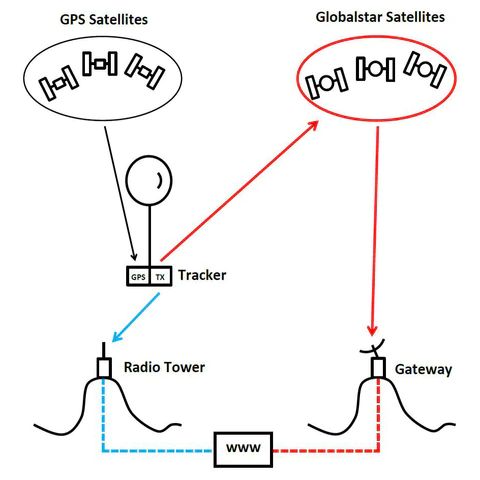
\includegraphics[width=0.4\textwidth]{gps_relay}
  \caption{GPS Relay Tracking \cite{site-highaltitudescienceTrackingWeather}}
  \label{fig:gps_relay}
\end{figure}

The major disadvantage of this method is the additional PocketQube hardware required. Not only does it need an antenna capable of communicating with one of the external networks, but it requires a GPS receiver, and a ground-station system if realtime data collection is needed. This type of tracking works well if the satellite is physically close to the external network satellites, or if the ground station does not need to communicate in realtime, but merely needs access to location of the satellite (e.g. in a homemade cellphone balloon satellite launch). A further disadvantage of this method is the need for a paid subscription to access the external network.


\subsection{Radio}
Radio tracking can be done when the satellite itself transmits radio waves. Techniques which provide simple direction pointing make use of the electromagnetic signal strength to point the ground station correctly. To initially find the satellite, the entire sky can be scanned or an initial guess can be provided. From there, periodic \textit{radius scanning} can be used to track the signal within a certain portion of the sky, or more advanced techniques such as \textit{conical scanning} can be used.